%++++++++++++++++++++++++++++++++++++++++
% Don't modify this section unless you know what you're doing!
\documentclass[letterpaper,11pt]{article}
\usepackage{tabularx} % extra features for tabular environment
\usepackage{amsmath}  % improve math presentation
\usepackage{graphicx} % takes care of graphic including machinery
\usepackage[margin=1.3in,letterpaper]{geometry} % decreases margins
\usepackage{cite} % takes care of citations
\usepackage[final]{hyperref} % adds hyper links inside the generated pdf file
\usepackage{titlesec}
\usepackage{verbatim}
\usepackage{ragged2e}
\usepackage{amssymb}
\usepackage{tikz}
\usetikzlibrary{calc}
\tikzset{axis line style/.style={thin, gray, -stealth}}
\newcommand*{\TickSize}{2pt}
\setcounter{secnumdepth}{3}
\newtheorem{theorem}{Theorem}[section]
\newtheorem{property}{Property}[theorem]
\newtheorem{lemma}{Lemma}[theorem]

\makeatletter
\def\BState{\State\hskip-\ALG@thistlm}
\makeatother
\hypersetup{
	colorlinks=true,       % false: boxed links; true: colored links
	linkcolor=blue,        % color of internal links
	citecolor=blue,        % color of links to bibliography
	filecolor=magenta,     % color of file links
	urlcolor=blue
}
\newcommand\given[1][]{\:#1\vert\:}
\usepackage{listings}
\usepackage{array}
\usepackage{diagbox}
\usepackage{multicol}
\lstset{
  basicstyle=\ttfamily,
  mathescape
}
\usepackage{caption}
\usepackage{hyperref}

\usepackage{fvextra} % loads also fancyvrb
\usepackage{xpatch}

\DeclareMathVersion{ttmath}
\DeclareSymbolFont{latinletters}{OT1}{\ttdefault}{m}{n}
%\SetSymbolFont{latinletters}{ttmath}{OT1}{\ttdefault}{m}{n}
\SetSymbolFont{letters}{ttmath}{OML}{ccm}{m}{it}
\SetSymbolFont{symbols}{ttmath}{OMS}{ccsy}{m}{n}
\SetSymbolFont{largesymbols}{ttmath}{OMX}{ccex}{m}{n}

\newcommand{\changeletters}{%
  \count255=`A
  \advance\count255 -1
  \loop\ifnum\count255<`Z
    \advance\count255 1
    \mathcode\count255=\numexpr\number\symlatinletters*256+\count255\relax
  \repeat
  \count255=`a
  \advance\count255 -1
  \loop\ifnum\count255<`z
    \advance\count255 1
    \mathcode\count255=\numexpr\number\symlatinletters*256+\count255\relax
  \repeat
  \count255=`0
  \advance\count255 -1
  \loop\ifnum\count255<`9
    \advance\count255 1
    \mathcode\count255=\numexpr\number\symlatinletters*256+\count255\relax
  \repeat
}

\xapptocmd{\ttfamily}{\mathversion{ttmath}\changeletters}{}{}
%++++++++++++++++++++++++++++++++++++++++


\begin{document}

\title{\textbf{Practical Network Defense}\\ \bigskip \large Second Assignment - University ``La Sapienza"}
\date{2020-13-06}
\author{\textbf{Group 27}: Nicola Bartoloni 1909908 - Valerio Trenta 1856471}
\maketitle

\section{Scope and Initial Considerations}
The scope of this assignment is to setup a \textbf{Virtual Private Network} through \textbf{OpenVPN} in \textbf{OPNSense} to allow three authenticated \textit{Road Warriors} to access the internal subnetworks of \textbf{ACME Co.}, and to grant the usage of a \textbf{proxy server} on machine located at \textbf{100.100.6.3} -  which corresponds to domain \textbf{proxy.acme.group27} to the very same authenticated internal clients of the network to reach the \textbf{WAN} outside the \textbf{Main Firewall}.\\
Since these tasks are going to allow connections from the outside - even if authenticated and thus probably secured - it is a good idea to make sure, as a first step, that every user on each of the internal machines is protected by a strong password, and we will probably also have to confirm that the SSH protocol on each machine behaves as we expect it to behave - some of the \textit{root} accounts are already disabled by SSH on some machines, but some are still accepting connections based on basic authentication.\\
The next paragraphs will only deal with the two services we want to setup in the target network - \textbf{VPN} and \textbf{proxy server}.

\newpage
\section{Infrastructure Setup}
We identify four main services which require machine-to-machine communication and, thus, are susceptible to the firewall rules that we'll define:\\
\begin{itemize}
\item an \textbf{Apache} web server reachable through \textbf{TCP} ports \textbf{80} (HTTP) and \textbf{443} (HTTPS) at \textbf{100.100.6.2};
\item a \textbf{DNS service} reachable through standard \textbf{UDP} port \textbf{53} at \textbf{100.100.1.2};
\item a \textbf{rsyslog at logserver} which we will make reachable through standard \textbf{UDP} port \textbf{514} at \textbf{100.100.1.3};
\item a \textbf{proxy server} reachable through port \textbf{3128} at \textbf{100.100.6.3}, to be configured later on Assignemnt 3.
\end{itemize}

We thus identify two new subnetworks: the \textbf{Internal Servers} subnetwork \textbf{100.100.1.0$/$24} and the \textbf{DMZ} subnetwork \textbf{100.100.6.0$/$24}, and for the sake of defining the scope of this assignment and the setup of the whole infrastructure, we should also consider two additional details:\\
\begin{itemize}
\item One of the four services - web server - is already setup and running in the system: it does not need to be configured or launched;
\item the \textbf{proxy server} is to be configured on the next assignment: for now, knowing from the \textbf{zentyal} portal that it is provided on port 3128 is enough.
\end{itemize}

This leaves us with the only \textbf{DNS service} to be configured at the moment, and the \textbf{rsyslog} process at \textbf{logserver} and at each of its clients to be defined later. The first step has been performed by following the instructions provided with the assignment: by accessing the \textbf{zentyal} portal at \textbf{100.100.1.2} on port \textbf{8843} - credentials have been changed - we added as forwarders the suggested IP addresses and specified the domain name - \textbf{acme.group27}. Then, the file located at \textbf{$/$etc$/$zentyal$/$dns.conf} on the aforementioned machine was modified including the target subnetworks (Clients and DMZ, that are the ones which will exploit the service).\\
At this point, pairs of IP addresses and hostnames were specified in the portal, so that the well-known machines of the network can now be associated with the following names:\\
\begin{itemize}
\item \textbf{kali}.acme.group27;
\item \textbf{watchdog}.acme.group27;
\item \textbf{dc}.acme.group27;
\item \textbf{web}.acme.group27;
\item \textbf{proxy}.acme.group27;
\item \textbf{coffee}.acme.group27;
\end{itemize}

also, as suggested in the assignment, the external services machines were provided with an external DNS service such as 8.8.8.8 in their DHCPv4 configuration. Please notice also that the \textit{logserver} was not given a name since it is only meant to be accessed by the SPOCK environment or by SSH and is not offering any browser-related service - and the same reasoning could be applied to the first two machines, \textit{kali} and \textit{arpwatch}, which we could exclude from this pairing list.\\
Last step was to actually modify the \tetxbf{DHCPv4} settings in the two main routers to set the \textbf{dc} machine as the \textbf{DNS server} in the Internal Servers network, after having disabled the \textbf{Service Unbound DNS} in both routers.\\
Keep also in mind that some of the machines with predefined IP addresses (fixed, not assigned by DHCP service) had either to be configured externally, or had to have their \textit{$/$etc$/$resolv.conf} file re-configured by modifying the IP address of their nameserver (for instance, Proxy and Kali machines).\\
The \textbf{DNS service} configuration is tested in section 5.

\subsection{Log server}
The \textbf{rsyslog} service at \textbf{logserver} was configured by modifying the file \textit{$/$etc$/$rsyslog.conf}, whose lines about \textbf{TCP} remote service were uncommented so that the service is listening on \textbf{TCP} port \textbf{514} for log messages to record from its clients. Then, a \textbf{template} was defined in this config file, so that for every log message that is received, the service records it under path \textit{$/$var$/$log$/$machine$/$process.log} - e.g., when process \textbf{login} from \textbf{webserver} machine sends a log message to the \textbf{logserver}, it is recorded under $/$webserver$/$login.log under the logging directory.\\
Then, for each \textbf{client} of the service, the very same config file was modified - so for every machine on \textbf{DMZ} and \textbf{Internal Servers} subnetworks, by appending to the end of the file \textit{*.* @@100.100.1.3:514} to specify that each log message from every process of the machine must be sent to the \textbf{logserver} through \textbf{TCP} protocol on port \textbf{514}. Figures \textbf{1} and \textbf{2} at page 8 show the outcome of this configuration.\\
The double \textit{@} character in the previous string strictly specifies that the protocol to be used is \textbf{TCP} and not \textbf{UDP}, since it is a best practice to exploit the first and not the latter when performing remote logging given that it is a more reliable and secure protocol. Please notice that we have also checked that, when further services were implemented in the machines that send remote logs to \textit{logserver} in the next assignments, these services are also logged under the corresponding directory of their machine - like \textit{fail2ban} service.

\begin{figure}[H]
\centering
\begin{minipage}{.5\textwidth}
  \centering
  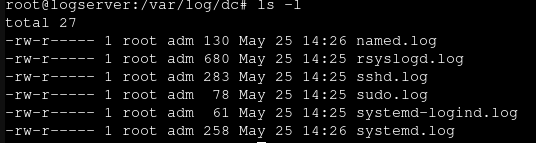
\includegraphics[width=1\textwidth]{logserver_dc.png}
  \caption[a]{Log files sent by 100.100.1.2 - dc machine.}\label{fig:1}
\end{minipage}%
\begin{minipage}{.5\textwidth}
  \centering
  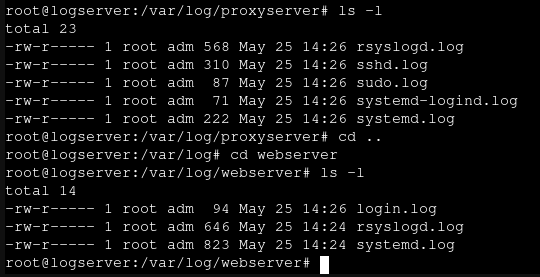
\includegraphics[width=1\textwidth]{logserver_dmz.png}
  \caption[a]{log files sent by machines in DMZ subnet.}\label{fig:2}
\end{minipage}
\end{figure}

\newpage
\section{Policy Evaluation}
The proposed policy targets the four services listed in the previous paragraph and a series of machines which will either exploit or provide the corresponding services.\\
The best way of interpreting and understanding this policy is given by its fifth line:\\
\begin{itemize}
\item \textit{"Anything that is not specifically allowed has to be denied"};
\end{itemize}

which suggests the \textit{white-listed} approach we have to adopt when defining the firewall rules: the policy is a list of \textbf{PASS} rules - meaning, rules that when matched will let the packet pass and continue its journey - while everything that doesn't match the rule has to be rejected, i.e. the packet must be dropped. Thus, we can devise a list of rules to apply at each of the two target routers and their corresponding effects on the network.\\

\textbf{Internal Router:}
\begin{itemize}
\item \textbf{Clients Interface}: only accept incoming packets on this interface with destination ports 80(HTTP), 443(HTTPS), 22(SSH), 53(UDP-DNS) and 3128(Proxy Service). Anything else will be discarder, since clients are not supposed to perform different actions and exploit different protocols than the aforementioned ones. For practical reasons, also packets on port 8443 (for \textbf{zentyal} panel service) are allowed - but this might be changed;
\item \textbf{Servers Interface}: only accept incoming packets on this interface with destination port 53(UDP-DNS) or 514(UDP-SYSLOG, only if coming from \textbf{DMZ subnet}) and on port 22(SSH) only if coming from the \textbf{Clients subnet}, otherwise discard. This means that the two servers can only be reached by Clients or DMZ subnetworks, and only for the services that they provide (SYSLOG, DNS, SSH);
\end{itemize}

\textbf{Main Router:}
\begin{itemize}
\item \textbf{Internal Interface:} only accept incoming packets on this interface on ports 80(HTTP) and 443(HTTPS) between \textbf{Clients subnet} and \textbf{External services subnet}, or ports 22(SSH) and 3182(Proxy) between \textbf{Clients subnet} and \textbf{DMZ subnet}, or ports 53(UDP-DNS) and 514(UDP-SYSLOG) between \textbf{DMZ subnet} and \textbf{Internal services subnet}, otherwise discard. This means the Client host will only be able to reach the external web services, or the proxy to actually reach the WAN, and won't be able to do it directly by itself. Furthermore, SSH is eanbled for Client hosts to reach the \textbf{DMZ subnet} and the services offered by the \textbf{Internal servers} are reachable from the machines in the DMZ;
\item \textbf{DMZ Interface:} we want the proxy server to be able to reach the internet via HTTP$/$HTTPS protocol, so we specify that this interface has to accept incoming packets specifically from the \textbf{Proxy server} and with \textbf{any} destination address on ports HTTP$/$HTTPS, and the same goes (but reversed) for the \textbf{web server} which we want to be accessible on ports HTTP$/$HTTPS from the Internet. However, the \textbf{proxy service} itself must be only available for client hosts in the \textbf{Clients subnet}, so we should also specify that this interface should accept incoming packets on port 3182 of the Proxy machine with source address in the \textbf{Clients subnet}. The aforementioned rules for DNS/SYSLOG services in the Internal Services apply also here on this interface, while every other packet which is not \textit{white-listed} must be rejected;
\item \textbf{WAN Interface:} this interface should be the first line of prevention against intruders from the Internet, so it only has to accept - as specified by the policy - connections with destination port 80 or 443 on the \textbf{web server} machine in DMZ and connections to any other machine in the Internet on port 80 or 443 if they are initiated by the \textbf{Proxy} machine in DMZ: every other packet incoming on this interface should be rejected.
\end{itemize}

If implemented correctly, this policy should allow the Internal services to be exploited and reachable only by the \textbf{Clients or DMZ networks}, and it should also allow the client hosts in the \textbf{Clients} network to either reach the \textbf{external web services} or the Internet via the \textbf{Proxy service} to be configured in the next assignment, being this service in the \textbf{DMZ} the only one able to actually initiate connections with Internet, while the \textbf{web server} should be the only machine which can accept connections initiated by someone else outside our target network.\\
Notice that this may not be the only possible setup to actually implement the policy, and we will deal with this in the next paragraph.

\newpage
\section{Policy Implementation}
While evaluating the policy in the previous paragraph, we have already proposed a high-level description of the rules to be implemented at each interface of the two firewalls. Notice that, for instance, the rules we applied at the \textbf{Internal interface} of the \textbf{Main Router}, could have also been applied, instead, at the \textbf{External interface} of the \textbf{Internal Router} or, to have a complete in-depth defence, the same rules could have been applied at both interfaces - which could also be the best solution in order to prevent bad scenarios like the failure of one of the two firewalls.\\
Also, there is another interesting fact about OPNSense Firewall configuration: it tracks connections by default, so that every packet in a TCP connection which has already been \textit{established} and has been accepted, is automatically accepted (\textit{pass} action) by default. This means that if we set a rule to allow machine A to ping machine B through ICMP protocol and then another one which rejects by default any other connection on that interface, since OPNSense by default applies to the packet the very first rule that matches, machine B's response will be automatically accepted too by the firewall, while if machine B initiates a new connection by pinging machine A, the firewall will not allow it - and we can verify this on the testing paragraph.\\
While implementing this policy, several \textbf{aliases} had to be defined in OPNSense's Firewall service at each of the two routers. These aliases could either be single hosts or single subnetworks, which were in some cases already present by default. This way, machines or subnets that were allowed to send or receive specific packets on an interface were addressed more precisely, and we were able to make important distinctions between hosts in the same subnet but with different policies - i.e., \textbf{Web Service} and \textbf{Proxy Service} in the \textbf{DMZ subnet}, or the two internal services \textbf{DNS} and \textbf{Log}.\\
These are the rules that were specified on each of the two routers:\\
\textbf{Internal Router:}
\begin{itemize}
\item \textbf{Clients Interface}: only accept incoming packets on this interface with destination ports 80(HTTP), 443(HTTPS), 22(SSH), 53(UDP-DNS) and 3128(Proxy Service). Anything else will be discarder, since clients are not supposed to perform different actions and exploit different protocols than the aforementioned ones. For practical reasons, also packets on port 8443 (for \textbf{zentyal} panel service) are allowed - but this might be changed;
\item \textbf{Servers Interface}: only accept incoming packets on this interface with destination port 53(UDP-DNS) or 514(TCP-SYSLOG, only if coming from \textbf{DMZ subnet}) and on port 22(SSH) only if coming from the \textbf{Clients subnet}, otherwise discard. This means that the two servers can only be reached by Clients or DMZ subnetworks, and only for the services that they provide (SYSLOG, DNS, SSH);
\item \textbf{External Interface:} we can either set the same rules of the \textbf{Main Router}'s \textbf{Internal Interface} to have a more robust setup, or leave this with its default configuration;
\end{itemize}
\textbf{Main Router:}
\begin{itemize}
\item \textbf{Internal Interface:} only accept incoming packets on this interface on ports 80(HTTP) and 443(HTTPS) between \textbf{Clients subnet} and \textbf{External services subnet}, or ports 22(SSH) and 3182(Proxy) between \textbf{Clients subnet} and \textbf{DMZ subnet}, or ports 53(UDP-DNS) and 514(TCP-SYSLOG) between \textbf{DMZ subnet} and \textbf{Internal services subnet}, otherwise discard. This means the Client host will only be able to reach the external web services, or the proxy to actually reach the WAN, and won't be able to do it directly by itself. Furthermore, SSH is eanbled for Client hosts to reach the \textbf{DMZ subnet} and the services offered by the \textbf{Internal servers} are reachable from the machines in the DMZ;
\item \textbf{DMZ Interface:} we want the proxy server to be able to reach the internet via HTTP$/$HTTPS protocol, so we specify that this interface has to accept incoming packets specifically from the \textbf{Proxy server} and with \textbf{any} destination address on ports HTTP$/$HTTPS, and the same goes (but reversed) for the \textbf{web server} which we want to be accessible on ports HTTP$/$HTTPS from the Internet. However, the \textbf{proxy service} itself must be only available for client hosts in the \textbf{Clients subnet}, so we should also specify that this interface should accept incoming packets on port 3182 of the Proxy machine with source address in the \textbf{Clients subnet}. The aforementioned rules for DNS/SYSLOG services in the Internal Services apply also here on this interface, while every other packet which is not \textit{white-listed} must be rejected;
\item \textbf{WAN Interface:} this interface should be the first line of prevention against intruders from the Internet, so it only has to accept - as specified by the policy - connections with destination port 80 or 443 on the \textbf{web server} machine in DMZ and connections to any other machine in the Internet on port 80 or 443 if they are initiated by the \textbf{Proxy} machine in DMZ: every other packet incoming on this interface should be rejected;
\item \textbf{External services Interface:} since anything that is not specifically allowed must be denied, this interface should only allow external clients to establish a connection with their DNS service and an HTTP$/$HTTPS connection with the internal clients of our network, while anything else (including HTTP$/$HTTPS with \textbf{WAN} or SSH with internal clients) should not be allowed.
\end{itemize}

\textit{Please notice that for practical reasons, hosts in the Clients subnetwork have also been granted the possibility to access the two routers via their HTTP service.} This is not specified by the policy and thus should not be allowed, but since we are still implementing the whole infrastructure, we need access to this service from this subnetwork. At the end of the whole process, this rule should be disabled.

\newpage
\section{Tests}
Tests that we run on both the two services aimed at verifying their correct behavior - i.e., that the two services were actually confgiured correctly so to be exploited as desired by non-malicious users - and that their setup does not hold a negative impact on the policy implemented in the previous assignment - i.e., the services can be only exploited by authenticated users under certain already mentioned conditions.

\subsection{Testing the VPN}
The \textbf{OpenVPN} service implemented on the \textbf{Main firewall} must be exploited only by an \textit{authenticated user} - that is, a user who owns \textit{three distinct credentials} in order to prove its identity and correctly gain access to the service. These three credentials are: the \textbf{.ovpn} file provided by the \textbf{OPNSense} portal correctly specifying the \textbf{valid cryptographic parameters} to authenticate the user on the \textbf{OpenVPN server}. This file holds the parameters that we previously showed, like port number, authentication type and the cryptographic functions to be arranged during the handshake between client and server, as pictured in \textbf{figure 7}.

\begin{figure}[!htb]
\centering
\begin{minipage}{.33\textwidth}
  \centering
  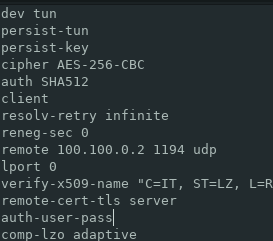
\includegraphics[width=1\textwidth]{ovpnParams.png}
  \caption[a]{Parameters in the .ovpn client file.}\label{fig:7}
\end{minipage}%
\end{figure}

Along with these parameters, the file also holds two different \textbf{keys}, one being the \textbf{certificate} for client to server authentication, the other being the \textbf{2048 bit OpenVPN static key} provided during the \textbf{TLS authentication}.\\
The other two credentials are the pair \textbf{(username, password)} specified under the settings of the \textbf{OPNSense} pannel - e.g., \textbf{Becca} as username and \textbf{password} as her password - and, furthermore, a \textbf{six characters token} provided by the \textbf{Google Authenticator}, which is a \textbf{One Time Password} different for each of the three users to be provided along the user's own static password during the basic authentication phase.\\
Once the \textbf{OpenVPN} terminates the intialization and the user authenticates successfully, he can exploit the new \textbf{tunnel} to gain access to the machines under the \textbf{Clients subnetwork} as requested by the assignment, through the \textbf{SSH} protocol on its own machine located in the \textbf{WAN} - once the \textbf{SSH} service has been enabled on the client's machines and routing has been appropriately configured on the local machine. This is the only operation that the \textbf{road warriors} are enabled to perform - they do not have access to the other subnetworks in the whole network, but we should stress the point that, once they gain access to one of the machines in the \textbf{Clients subnetwork}, they do have access to any other machine in the internal and DMZ subnet, which should actually be a desired feature.\\
\textbf{Figure 8} pictures the successful remote access of user \textbf{Becca} to the \textbf{kali machine} via the \textbf{OpenVPN service}. As far as we know, the only vulnerability that is introduced in the network with this service, is that now the \textbf{Main firewall} accepts connections on port \textbf{1194} on the \textbf{WAN} interface, and that the machines in the \textbf{Clients subnetwork} now accept connections with protocol \textbf{SSH} on \textbf{port 22} if and only if the request is coming from the \textbf{OpenVPN} tunnel - that is, only authenticated users should be actually able to login via \textbf{SSH} on those machines from the \textbf{WAN}.\\

\begin{figure}[!htb]
\centering
\begin{minipage}{.80\textwidth}
  \centering
  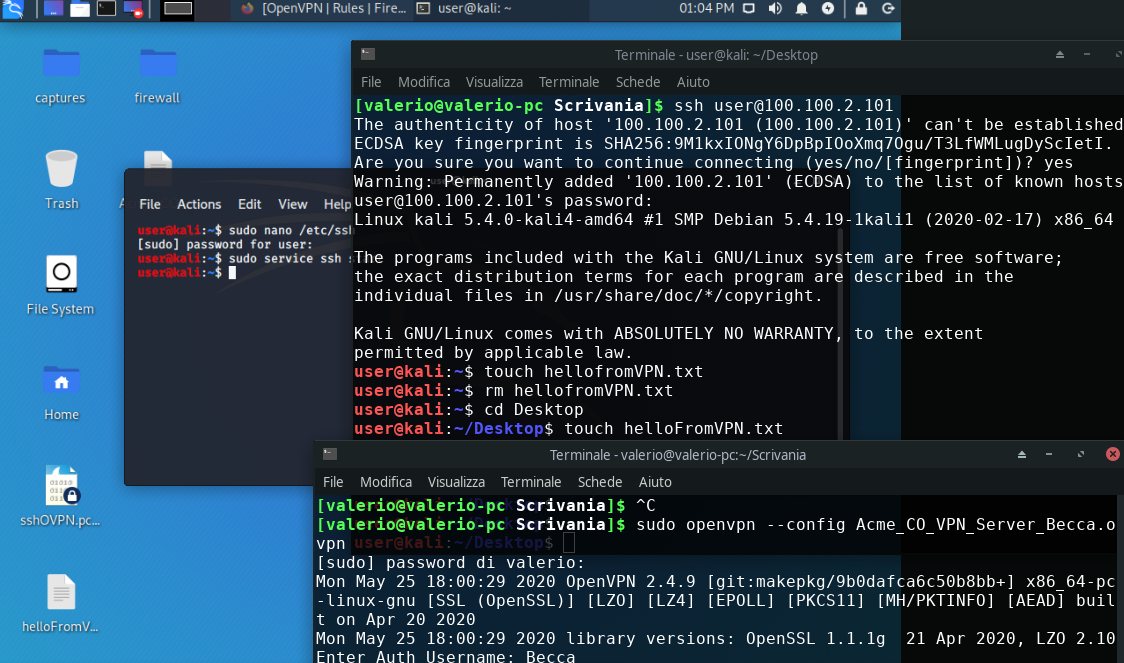
\includegraphics[width=1\textwidth]{OVPNaccessViaSSH.png}
  \caption[a]{User Becca accessing the Kali Machine via OpenVPN-SSH.}\label{fig:8}
\end{minipage}%
\end{figure}

\subsection{Testing the Proxy service}
We want the \textbf{squid proxy service} on the \textbf{proxy machine} to accept only users that have authenticated and are located in the \textbf{Clients subnetwork}, thus connections coming from a different subnetwork or the \textbf{WAN} are rejected a priori. In the \textbf{Kali machine}, we setup \textbf{Firefox browser} preferences so that it connects to the \textbf{proxy machine} requesting the \textbf{squid} service on port \textbf{3128} for every HTTP or HTTPS connection but those that have destination in the \textbf{Internal}, \textbf{External services} or \textbf{DMZ} subnetworks - \textit{manual configuration}. The figures below picture the desired behavior of both the services and the client's browser, which is now able to \textit{go out} in the \textbf{WAN} once the user is authenticated.\\

\begin{figure}[!htb]
\centering
\begin{minipage}{.5\textwidth}
  \centering
  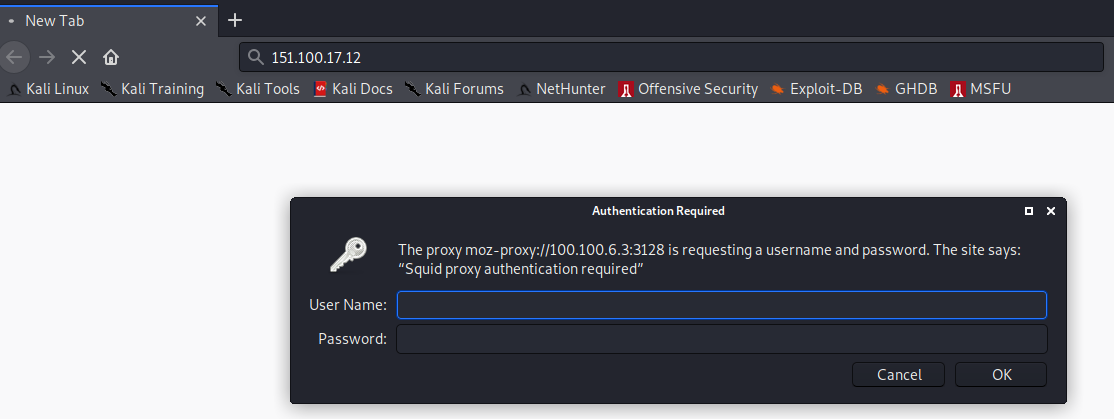
\includegraphics[width=1\textwidth]{proxyAuth.png}
  \caption[a]{Authentication procedure in the Kali machine's browser.}\label{fig:9}
\end{minipage}%
\begin{minipage}{.5\textwidth}
  \centering
  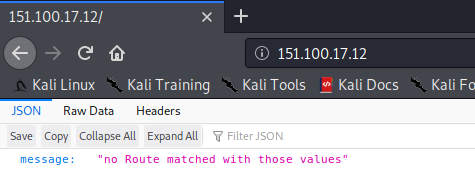
\includegraphics[width=1\textwidth]{proxyAuthed.png}
  \caption[a]{Successfully authenticated user can exploit proxy to display web pages outside of the network.}\label{fig:10}
\end{minipage}%
\end{figure}

\newpage
\section{Final remarks}
The testing phase showed us that the policy, if correctly interpreted, was implemented as specified by the assignment.\\
Some extra measures could have been taken, and they are very similar to the ones we have seen in the first assignment: we need to perform Linux hardening via sudo and hardening of the SSH protocol for all the machines in the DMZ and Internal Service subnetworks, and we need to change the default passwords for services such as \textbf{Zentyal} too and for users on the machines as well.\\
We should also stress the fact that, even if we found out that some of the machines had the SSH login via their \textit{root} account disabled by default, the scope of this assignment was to focus mainly on the \textbf{firewall rules} to be defined to achieve our goals and implement the given policy: this means that link$-$layer attacks were not taken into consideration, and this may be a critical vulnerability in our network. indeed, notice that every machine can be accessed through SSH or other protocols by any other machine on its same subnetwork - i.e., \textit{dc} can access \textit{logserver} through any protocol. This is because the rules we defined to implement our policy are placed on the two firewall$-$routers, which obviously do not handle packets exchanged between hosts in the same subnetwork: to overcome this issue, probably some extra rules should also be defined locally on each machine via \textit{iptables} - but this was out of our scope for this assignment.\\
We should also mention the fact that the \textbf{UDP} protocol was chosen to implement the \textbf{rsyslog} service, which could be also implemented through \textbf{TCP} protocol - commonly considered more secure - and maybe forced to exploit secure channels. Again, our goal here was to enable the service and enforce the policy via firewall rules, but we should stress the fact that just by exploiting TCP, this service may be hardened.\\
Also, as a last step, when the whole configuration going on in these assignments is over, we should at least enable only one machine in the \textbf{Clients} subnetwork - the \textbf{Kali} machine, probably - to connect via HTTP service to the two routers, for administration and practical reasons, so as we mentioned in the previous paragraphs, the rule enabling these connections should be actually disabled as a last step.

\newpage

\end{document}
